\chapter{Discussion}\label{chap:discussion}

We found very little freely available research papers about ECS based game engines, that also have an actual implementation. This makes our contribution unique in this field, as it describes the concept and implementation of a working game engine using the ECS architecture and leveraging the Effekt language's features.

The idea to use the ECS architecture was not present from the start, but other solutions to a generic `world'/`scene' object management system seemed hard to implement in Effekt. Considering that, the ECS architecture seemed to fit our needs and was promising to implement using effects and handlers. We tried multiple architectures to organize the game engine and especially the ECS. The query API needed multiple iterations, as one reason for the previous system not working, was the lack of bidirectional effects in an operation mentioning its own effect. This is would be a kind of "recursive bidirectional effect" and is not (yet) supported in Effekt. The component effect also had multiple arrays at one point, stored in a map from archetype ID to component values. This allowed for sequential iteration of components, as every component of every archetype had its own array in the same order. This was more complicated to implement, though, and therefore was abandoned during a rework of the ECS.

\section{Leveraging the Effekt Language}

The Effekt language with its effect system provides many features required or useful for our game engine and API implementation.

\begin{description}
\item[Bidirectional effects] are required for any effect that uses another effect at the call site of the operation. This includes the |EntityManager| effect with all its API effect operations, which need a |Component[T]| effect handled at the call site of the operation, as they are not yet available when creating the |World| and therefore handling the |EntityManager|. This is also required for the |Query| effect to add (optional) components to it.
\item[Executing handler code after resumption] is required to make deferred modification inside the systems possible, as these |systemEntityManager| operations need to register their modification after the |resume| call. Otherwise, systems could run endlessly if modifications were applied during iteration.
\item[Existential types] are required to make dynamic archetypes possible. Otherwise, there would be no way to add components without specifying all previous components in the set component function call type signature and no way to destroy entities without specifying all components of it in the destroy function call type signature. These components can only be destroyed by storing the typed component stores inside existential types that can remove values from it without needing its actual type signature from the outside.
\item[Named handlers] are required to have multiple |CompIter| handlers at the same time, which are needed to add multiple (optional) components to a query. They are later used during iteration of the query to get and set the current value of these (optional) components.
\item[Contextual effect polymorphism] is required to be able to use any local effect handler inside of systems, without the |System| effect knowing anything about what local effects/variables the actual system body uses.
\end{description}

\section{Game Engines and ECS as Domain Specific Languages}

Domain specific languages (DSLs) are languages designed for a specific domain, restricting semantics and syntax to the level needed for the specific domain, as opposed to general purpose programming languages~\cite{hudak1997domain}. Some examples for this are HTML and LaTex for document layout, SQL for databases and the OpenGL API for (3D) graphics.

The domain of game engines is game development. As game engines are based on specific core systems, they have a specific architecture and therefore API for the user. This API of game engines can also be seen as a domain specific language. Especially for ECS based game engines, this architecture has a very specific way of defining the game world and its transformations.

Having specialized semantics for entities, components, resources, systems, queries and the world makes it ideal to be defined as a domain specific language. The syntax of the implemented API together with the Effekt syntax then define the syntax of this DSL.

\section{Restricting API Usage}

Currently, the Effekt language does not provide visibility modifiers. It does offer modules, but we chose instead to prefix all function/operation names that should never be called from library user code with `internal'. Using an `internal' module would still allow the library user to call these, so modules would not be able to limit the API usage either.

Apart from calling functions/operations with the `internal' prefix, there are still other ways to use the API that are not intended. One of these is to handle multiple |World|s, registering components multiple times or handling other ECS related effects manually. This does not break the program most of the time, but can be very confusing. For example, a second world would be completely separate from the first one and used until it is out of scope, but the first world will not change while a second one is handled. Registering a component for the second time will give it another type ID, which will then be used until that |Component| effect is out of scope. This second handler of the component, however, will not use the same storage as the first and archetypes using the second |Component| handler will be different from ones using the first.

The last major unintended API usage possibility comes from the simple fact that an effect operation can be wrapped in a local function where the effect is handled. This allows the function to not require that effect anymore, while still using the handler from the definition site directly. As explained earlier, deferred modification inside systems is made possible by handling an alternative |EntityManager| implementation (|systemEntityManager|) inside every system body to avoid infinite iteration and more. This can be circumvented by creating a function that captures the |createEntity| effect operation from outside a system using the normal |EntityManager|, but then calling that function inside a system, where it is now independent of the local deferred |EntityManager|.

\newsavebox{\localfunctionwrap}
\begin{lrbox}{\localfunctionwrap}
\begin{lstlisting}
...
  def localCreateEntity() = {
    // Uses the direct/raw EntityManager:
    do createEntity()
  };

  with def query = query();
  with system() {
    query.foreach() { (_) =>
	  // Skips the deferred EntityManager (do createEntity())
	  // and creates the entity immediately
      localCreateEntity()
    }
  }
...
\end{lstlisting}
\end{lrbox}

\begin{figure}[h!]
\centering
\tikzstyle{box}=[rectangle,draw,rounded corners=0.5ex,minimum height=0.5cm,minimum width=1.5cm]
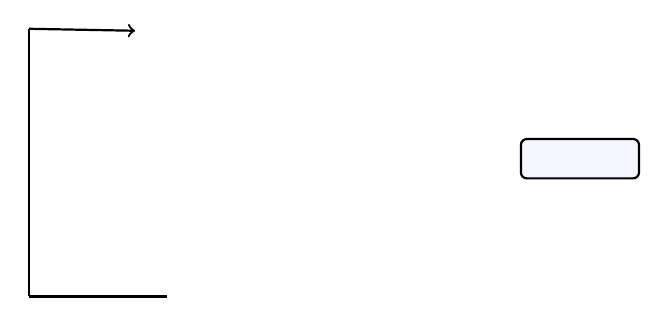
\begin{tikzpicture}[thick,font=\sf\scriptsize]
\node[box,fill=blue!4,align=center] at (0,0) {\usebox{\localfunctionwrap} \hspace*{.5mm}};
\draw[-] (-5.25,-1.75) -- (-7,-1.75);
\draw[-] (-7,-1.75) -- (-7,1.65);
\draw[->] (-7,1.65) -- (-5.65,1.625);
\end{tikzpicture}
\caption{Wrapping the EntityManager in a local function to directly create entities in a system, instead of normally deferring creation.}
\label{fig:localfunctionwrap}
\end{figure}

In \Cref{fig:localfunctionwrap}, an example is given, showing how this problem can occur. If inside the system, a new entity would be created with the |do createEntity()| operation directly, this system would double the entity count every time it ran, as it would create a new entity for every existing entity. This then works, as the actual entity creation is deferred until after the system has run. In this example, though, we use the local function that captured the direct/raw |EntityManager| from outside the system and create an entity with that. This makes the system iterate infinitely, as entities are created directly and are then already included during iteration.

The first issue can be fixed as soon as a proper system for visibility/access restriction is implemented in Effekt. The second issue of capturing an effect operation in a function can not be solved with the current concept of the Effekt language, as this builds on top of some of the core concepts of Effekt. For this, a complicated workaround would be needed to prevent this, or the library needs to specify that this is not allowed. One possibility could be requiring a boxed function for the system, which makes the function not able to use any local variables (regions) by explicitly stating it in the type signature. This would, however, limit the safe capabilities of systems and boxing might not be flexible enough for this solution.

\section{Query API and Drawbacks}

The initial plans for our query API was to specify the components and filters as generic types on query creation/handling and then iterate all the components via the query, not just the entity values themself. This turned out to not be feasible with the way the effect systems works. The current query API is quite verbose, including significant amounts of boilerplate code, but accomplishes the requirements in an easy-to-understand form. While easy to understand, the named handler syntax can need some getting used to.

The current query implementation in general is also not perfect, as it needs to completely recalculate their matches before the next iteration whenever any structural change was made. This means adding a component to one single entity makes all queries recalculate for the next frame. The recalculation is compromised of checking all archetypes whether they include all required components but none of the `without' filter components and creating an array for these matching archetype indices. This very conservative approach can be improved in multiple ways, as mentioned in the Conclusion, under `Future work'.

\section{Optimization and Indirect Component Access}\label{sec:indirectaccess}

Many ECS libraries choose to store all values of a component type in separate arrays per archetype, while some even split these up into chunks of a specific size and memory alignment (often 16 kB). In both cases, many of the components that are iterated sequentially are also stored next to each other. This makes them very cache friendly and generally fast to iterate.

Our ECS uses a single dynamic array to densely store \textit{all} values of one component type, and each archetype stores an additional array with indices into the component array for every entity of that archetype. This leads to one more indirection while iterating and nonsequential access of component values. While most production-ready or performance-focused ECS libraries would be significantly impacted by this, our library is for research and testing purposes. On one side, the Effekt language is not optimized for performance that much, especially the \textsf{js-web} target running on JavaScript. On the other side, the JavaScript runtime with its `just in time' \textit{jit} compiler does many, often not easily predictable optimizations, which can potentially lead to this indirection not incurring any significant runtime overhead. Considering those points, having the extra indirection for component iteration should not be a relevant slowdown while making the implementation simpler and easier to understand.

\section{Memory Problems With JavaScript Backend}\label{sec:memoryproblem}

During testing of the engine and developing a game for a case study, we came across a problem of the current way JavaScript handles looping functions and the Effekt implementation.

The only way to create a continuously looping function in Effekt while giving control back to the JavaScript event loop to capture input events and more is to use the |wait| function, which uses the JavaScript |setTimeout| function. This makes the rest of the scope's code a lambda function given to the |setTimeout|, which makes the memory allocated per-frame currently not be garbage collected. While running the case study `Snake' game, this leads to the used memory constantly increasing, crashing the game after around one minute of gameplay.

Without modifying the Effekt language, this would need a complicated workaround, which could be done in future work, as mentioned in the \Cref{chap:conclusion}, under `Future work'.
